\documentclass[11pt,a4paper]{article}

% ----------------------------------------------------------------------
% Packages
% ----------------------------------------------------------------------
\usepackage[utf8]{inputenc}
\usepackage[T1]{fontenc}
\usepackage{lmodern}
\usepackage[margin=2.4cm]{geometry}
\usepackage{amsmath}
\usepackage{amssymb}
\usepackage{graphicx}
\usepackage{booktabs}
\usepackage{xcolor}
\usepackage{listings}
\usepackage{caption}
\usepackage{subcaption}
\usepackage{float}
\usepackage{fancyhdr}
\usepackage{tikz}
\usepackage[hidelinks]{hyperref}

% ----------------------------------------------------------------------
% Colors and code style
% ----------------------------------------------------------------------
\definecolor{dauphineblue}{RGB}{0,81,186}
\definecolor{codebg}{RGB}{245,245,245}
\definecolor{codekw}{RGB}{0,81,186}
\definecolor{codecomment}{RGB}{90,110,90}

\lstset{
    basicstyle=\ttfamily\footnotesize,
    backgroundcolor=\color{codebg},
    keywordstyle=\color{codekw}\bfseries,
    commentstyle=\color{codecomment}\itshape,
    stringstyle=\color{red!60!black},
    breaklines=true,
    showstringspaces=false,
    frame=single,
    rulecolor=\color{gray!40},
    framesep=4pt,
    aboveskip=8pt,
    belowskip=6pt,
    language=Java,
}

\lstdefinestyle{pseudo}{
    basicstyle=\ttfamily\footnotesize,
    backgroundcolor=\color{codebg},
    keywordstyle=\color{codekw}\bfseries,
    morekeywords={if,then,else,while,for,each,do,return,push,pop,add,not,and,goal},
    frame=single,
    rulecolor=\color{gray!40},
}

% Define an "Algorithm" float so algorithm blocks are labeled "Algorithm N"
% rather than "Listing N". Uses the float package (no extra dependency).
\floatstyle{plain}
\newfloat{algorithm}{htbp}{loa}
\floatname{algorithm}{Algorithm}

% ----------------------------------------------------------------------
% Header and footer
% ----------------------------------------------------------------------
\pagestyle{fancy}
\fancyhf{}
\renewcommand{\headrulewidth}{0.4pt}
\lhead{\small Artificial Intelligence and Reasoning}
\rhead{\small Lab 1: Rubik's Cube Solver}
\cfoot{\small \thepage}

\setlength{\parskip}{0.45em}
\setlength{\parindent}{0pt}

% ======================================================================
\begin{document}

% ======================================================================
% TITLE PAGE (not counted in the 12 pages)
% ======================================================================
\begin{titlepage}
\centering
\vspace*{2cm}

{\Large \textbf{Universite Paris Dauphine, PSL}}\\[0.3cm]
{\large Master 1 MIAGE}\\[2.5cm]

{\color{dauphineblue}\rule{\linewidth}{1.2pt}}\\[0.4cm]
{\huge \textbf{Solving the Rubik's Cube}}\\[0.5cm]
{\LARGE with the A* Search Algorithm}\\[0.4cm]
{\color{dauphineblue}\rule{\linewidth}{1.2pt}}\\[1.5cm]

{\large \textit{Course: Artificial Intelligence and Reasoning}}\\[0.3cm]
{\large Lab 1, Project Report}\\[2.5cm]

{\large \textbf{Authors}}\\[0.3cm]
{\large Mathias CHEBBAH}\\[0.15cm]
{\large Lamine BETRAOUI}\\[0.15cm]
{\large Bouna SALL}\\[2cm]

\vfill
{\large June 2026}

\end{titlepage}

% ======================================================================
\section*{Abstract}

This report presents a program that solves the Rubik's Cube. We model the cube
as a search problem and we solve it with the A* algorithm seen in Lecture 2. We
first run a uniform cost search. We then add two admissible heuristics that guide
the search. The first heuristic relaxes the problem so that each sticker moves on
its own. The second heuristic relaxes it so that each piece moves on its own. We
measure how scrambled a cube can be while still being solved fast. The results
confirm the course: a good heuristic gives large savings, and A* runs out of
memory long before it runs out of time.

\tableofcontents
\vspace{0.6cm}

% ======================================================================
\section{Introduction}

A Rubik's Cube is a small cube. Each of its six faces holds nine colored
stickers. Every face can turn, which mixes the colors. The cube is solved when
each face shows a single color. Our goal is to write the "solve" button of a
cube simulator. Given any mixed cube, the program must return a list of moves
that brings it back to the solved state.

This problem fits the search framework of the course. A cube configuration is a
state. A quarter turn of a face is an action. The solved cube is the goal. Every
move costs one, so the shortest sequence of moves is the optimal solution. We
therefore use the search methods of Lecture 2. In particular we use A*, which
returns an optimal solution when its heuristic is admissible.

The report is organized as follows. Section 2 states the problem with the five
components of a search problem. Section 3 describes the classes of the program.
Section 4 explains A* and our implementation. Section 5 presents the two
heuristics and shows that they are admissible. Section 6 reports the experiments.
Section 7 concludes.

% ======================================================================
\section{Problem formulation}

\subsection{The cube and its representation}

We follow the Western color scheme. The solved cube shows white on the UP face,
yellow on DOWN, red on FRONT, orange on BACK, blue on LEFT and green on RIGHT.
Opposite faces are UP and DOWN, FRONT and BACK, LEFT and RIGHT. Each face is a
three by three matrix of characters. The characters are 'W', 'R', 'G', 'B', 'Y'
and 'O', as the statement requires. Figure~\ref{fig:net} shows the solved cube
and a scrambled cube drawn by our interface as an unfolded net.

\begin{figure}[H]
\centering
\begin{subfigure}{0.46\textwidth}
\centering
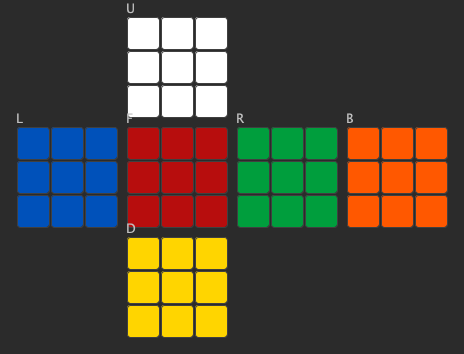
\includegraphics[width=\linewidth]{figures/cube_solved.png}
\caption{Solved cube.}
\end{subfigure}
\hfill
\begin{subfigure}{0.46\textwidth}
\centering
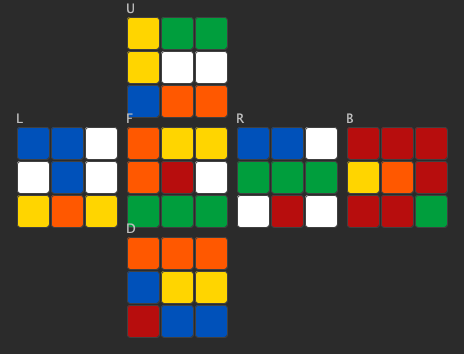
\includegraphics[width=\linewidth]{figures/cube_scrambled.png}
\caption{Cube after twelve random moves.}
\end{subfigure}
\caption{The cube shown by our interface as an unfolded net. The center of each
face never moves, so it keeps its solved color.}
\label{fig:net}
\end{figure}

Inside the program the 54 stickers are stored in one flat array. The matrix of a
face is a view over this array. Each face uses row and column indices from 0 to
2, as in the figure of the statement. To turn a face we must know where every
sticker goes. We place each sticker in a 3D frame, shown in
Figure~\ref{fig:axes}, where the cube is centered at the origin. A turn is then a
real rotation of one layer around an axis. This way the permutation is computed,
not typed by hand, so it cannot contain a wrong strip.

\begin{figure}[H]
\centering
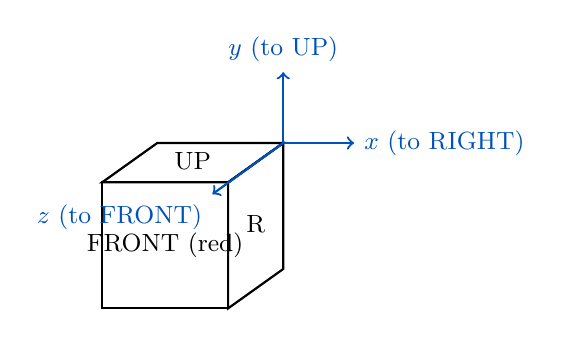
\begin{tikzpicture}[scale=1.0]
  % simple 3D-looking cube with axis labels
  \def\s{1.6}
  % front face
  \draw[thick] (0,0) rectangle (\s,\s);
  % top face (parallelogram)
  \draw[thick] (0,\s) -- (0.7,\s+0.5) -- (\s+0.7,\s+0.5) -- (\s,\s) -- cycle;
  % right face
  \draw[thick] (\s,0) -- (\s+0.7,0.5) -- (\s+0.7,\s+0.5) -- (\s,\s) -- cycle;
  % labels
  \node at (\s/2,\s/2) {\small FRONT (red)};
  \node at (\s/2+0.35,\s+0.27) {\small UP};
  \node[rotate=0] at (\s+0.35,\s/2+0.27) {\small R};
  % axes
  \draw[->,thick,dauphineblue] (\s+0.7,\s+0.5) -- (\s+1.6,\s+0.5) node[right]{\small $x$ (to RIGHT)};
  \draw[->,thick,dauphineblue] (\s+0.7,\s+0.5) -- (\s+0.7,\s+1.4) node[above]{\small $y$ (to UP)};
  \draw[->,thick,dauphineblue] (\s+0.7,\s+0.5) -- (\s+0.7-0.9,\s+0.5-0.65) node[below left]{\small $z$ (to FRONT)};
\end{tikzpicture}
\caption{The 3D frame used to compute the turns. The outward normal of each face
points along one axis. A clockwise turn rotates one layer by 90 degrees.}
\label{fig:axes}
\end{figure}

\subsection{The five components}

We define the search problem with the five components of Lecture 2.

\begin{itemize}
    \item \textbf{Initial state.} The scrambled cube given by the user.
    \item \textbf{Actions.} The twelve quarter turns. Six are clockwise (U, L, F,
          R, D, B). Six are counter clockwise (U', L', F', R', D', B').
    \item \textbf{Transition model.} Applying a turn produces a new cube. The
          result of an action permutes the stickers of one face and its belt.
    \item \textbf{Goal test.} The cube is solved when every face is uniform with
          its solved color.
    \item \textbf{Path cost.} Each move costs one. The cost of a path is its
          number of moves.
\end{itemize}

The state space is huge. A real cube has about $4.3 \times 10^{19}$ reachable
configurations. We cannot store them all. A* must therefore explore as few states
as possible, which is exactly why a good heuristic matters.

\subsection{The twelve actions}

Each action has an integer identifier, from 0 to 11, as in the statement. Table
\ref{tab:actions} lists them with their notation.

\begin{table}[H]
\centering
\small
\begin{tabular}{cccc@{\hspace{2cm}}cccc}
\toprule
Id & Method & Notation & Sense & Id & Method & Notation & Sense \\
\midrule
0 & turnUp    & U & clockwise & 6  & returnUp    & U' & counter \\
1 & turnLeft  & L & clockwise & 7  & returnLeft  & L' & counter \\
2 & turnFront & F & clockwise & 8  & returnFront & F' & counter \\
3 & turnRight & R & clockwise & 9  & returnRight & R' & counter \\
4 & turnDown  & D & clockwise & 10 & returnDown  & D' & counter \\
5 & turnBack  & B & clockwise & 11 & returnBack  & B' & counter \\
\bottomrule
\end{tabular}
\caption{The twelve actions and their identifiers.}
\label{tab:actions}
\end{table}

\subsection{Why this search is hard}

The course measures a search by three quantities. The branching factor $b$ is the
number of children of a node. The depth $d$ is the depth of the shallowest goal.
The maximum path length is $m$. For our problem $b$ is twelve, because each state
has twelve children. The number of nodes generated by a blind search grows like
$b^d$. With $b = 12$, even a small depth gives a very large tree. For example,
$12^7$ is more than thirty million. This is why a uniform cost search cannot go
deep, and why we need a heuristic.

\begin{table}[H]
\centering
\small
\begin{tabular}{lcc}
\toprule
Measure & Symbol & Value for our problem \\
\midrule
Branching factor & $b$ & 12 (twelve turns) \\
Worst case time  & $O(b^d)$ & exponential in the depth \\
Worst case space & $O(b^d)$ & the real limit we hit \\
\bottomrule
\end{tabular}
\caption{Complexity terms of the course applied to the cube.}
\label{tab:complexity}
\end{table}

% ======================================================================
\section{Program architecture}

The code is written in Java. We chose Java because the statement describes a
graphical interface, an interface for heuristics, and Java collections such as
the linked list. The classes follow the statement closely. They are grouped by
role, as Table~\ref{tab:classes} shows.

\begin{table}[H]
\centering
\small
\begin{tabular}{lll}
\toprule
Package & Class & Role \\
\midrule
model     & \texttt{Cube}                 & Six face matrices, the twelve turns, isSolved \\
model     & \texttt{Face}, \texttt{Color} & Faces, colors and their solved values \\
model     & \texttt{Move}                 & Notation and inverse of each action \\
search    & \texttt{State}                & A node of the search tree, with expand \\
search    & \texttt{Astar}                & The A* algorithm and the solve method \\
search    & \texttt{StateSet}             & The explored set, with add and contains \\
search    & \texttt{PriorityQueueState}   & The frontier, with push and pop \\
heuristic & \texttt{Heuristic}            & The heuristic interface, with value \\
heuristic & \texttt{HeuristicLabel}       & The sticker relaxation heuristic \\
heuristic & \texttt{HeuristicCube}        & The piece relaxation heuristic \\
ui        & \texttt{RubiksCubeSimulator}  & The interface and the solve button \\
\bottomrule
\end{tabular}
\caption{Main classes of the project, grouped by package.}
\label{tab:classes}
\end{table}

\subsection{The Cube class}

The \texttt{Cube} class models the game. It stores the 54 stickers and offers the
twelve turns and the \texttt{isSolved} test. The hard part is to know which
sticker moves where for each turn. Writing these tables by hand is error prone.
Instead, we give each sticker a position in 3D and a face normal. We then rotate
the affected layer with a real 90 degree rotation. We read the permutation back
from the rotated positions. This is correct by construction.

We checked the model with algebraic invariants. A turn followed by its inverse is
the identity. The same turn four times is the identity. A turn and three turns
the other way give the same result. The number of stickers of each color stays
nine. The classic sequence R U R' U' returns to the solved cube after exactly six
repetitions. All these tests pass.

\subsection{The State class}

A \texttt{State} is a node of the search tree. It stores the cube, the number of
actions from the root (the cost $g$), the parent state, the action used to reach
it, and the heuristic value $h$. The constructor computes $h$ once. The
\texttt{expand} method applies the twelve turns and returns the twelve children
in a linked list, as the statement asks. Algorithm~\ref{alg:expand} shows the
method.

\begin{algorithm}[H]
\caption{The expand method generates the twelve children.}
\label{alg:expand}
\begin{lstlisting}
public LinkedList<State> expand() {
    LinkedList<State> children = new LinkedList<>();
    for (int action = 0; action < 12; action++) {
        Cube next = cube.withAction(action);
        children.add(new State(next, nbrActions + 1, this, action));
    }
    return children;
}
\end{lstlisting}
\end{algorithm}

Each child keeps a reference to its parent and to the action that produced it.
These two fields, called \texttt{pere} and \texttt{actionPere} in the statement,
let us rebuild the full solution once the goal is reached. We compare two states
by their cube only. Two paths that reach the same configuration are therefore the
same state. This is what lets the explored set and the frontier remove
duplicates.

\subsection{The explored set and the frontier}

The \texttt{StateSet} class is the explored set. It offers \texttt{add} and
\texttt{contains}. It also keeps the smallest cost with which each configuration
was expanded. This lets A* skip a configuration already reached by a cheaper
path. The \texttt{PriorityQueueState} class is the frontier. It offers
\texttt{push} and \texttt{pop}. The \texttt{pop} method returns the state with
the smallest value $f = g + h$. The \texttt{push} method checks if the same
configuration is already in the frontier and keeps only the better one.

\subsection{The graphical interface}

The \texttt{RubiksCubeSimulator} class is the interface. It holds a cube and
draws it as the net of Figure~\ref{fig:net}. It has a \texttt{main} method that
creates the window. Its \texttt{actionPerformed} method reacts to every button.
There is one button per turn, a scramble button, a reset button, and the solve
button. There is also a small menu to pick the strategy.

When the user presses solve, the program runs A* on a copy of the cube. The
search runs on a background thread, so the window stays responsive. When the plan
is ready, the interface plays it move by move on the cube, like a short
animation. The log panel shows the plan, the number of expanded states, and the
time. While the search and the animation run, the move buttons are disabled, so
the user cannot change the cube under the solver. Figure~\ref{fig:gui} shows the
full window with a scrambled cube.

\begin{figure}[H]
\centering
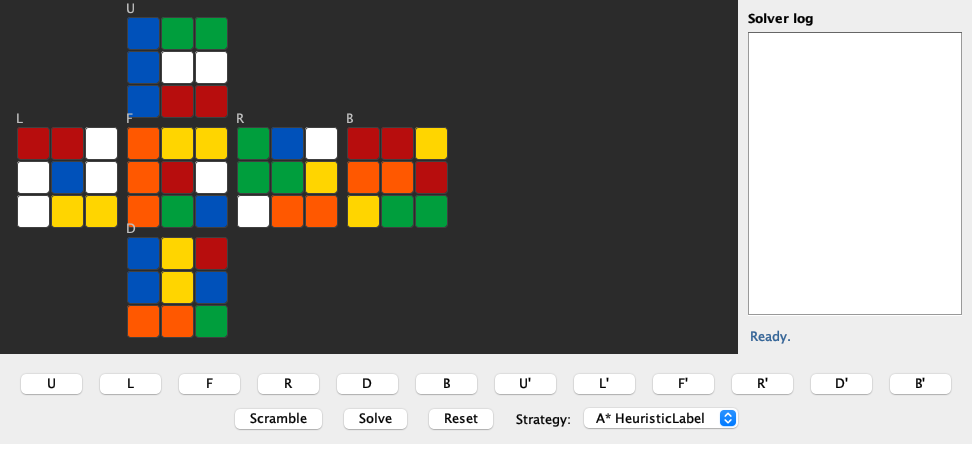
\includegraphics[width=0.96\linewidth]{figures/gui.png}
\caption{The simulator window. The cube net is on the left, the solver log on the
right, the twelve move buttons and the solve button below, with a menu to pick the
strategy.}
\label{fig:gui}
\end{figure}

% ======================================================================
\section{The A* algorithm}

\subsection{Principle}

A* is an informed search. It expands the node with the smallest evaluation
function
\[
f(n) = g(n) + h(n),
\]
where $g(n)$ is the cost from the start to $n$, and $h(n)$ estimates the cost
from $n$ to the goal. When $h$ is admissible, that is, when it never overestimates
the real cost, A* returns an optimal solution. With $h = 0$ the function $f$
becomes $f = g$, so A* behaves as a uniform cost search.

The course presents several search strategies. Table~\ref{tab:strategies}
compares the ones we use. The uniform cost search is complete and optimal but
blind. It explores by cost only. A* keeps the same guarantees but adds the
heuristic, so it looks toward the goal. This is why A* expands far fewer states
when the heuristic is good.

\begin{table}[H]
\centering
\small
\begin{tabular}{lccc}
\toprule
Strategy & Orders the frontier by & Optimal & Uses a heuristic \\
\midrule
Breadth first search & depth & yes (unit cost) & no \\
Uniform cost search  & $g$ & yes & no \\
Greedy best first    & $h$ & no & yes \\
A*                   & $f = g + h$ & yes (admissible $h$) & yes \\
\bottomrule
\end{tabular}
\caption{Search strategies of the course. We use uniform cost search and A*.}
\label{tab:strategies}
\end{table}

Figure~\ref{fig:tree} shows a small search tree. Each node carries its values
$g$, $h$ and $f$. A* always expands the leaf with the smallest $f$. A node that
looks cheap by $g$ alone may be skipped if its heuristic is large, and the other
way around.

\begin{figure}[H]
\centering
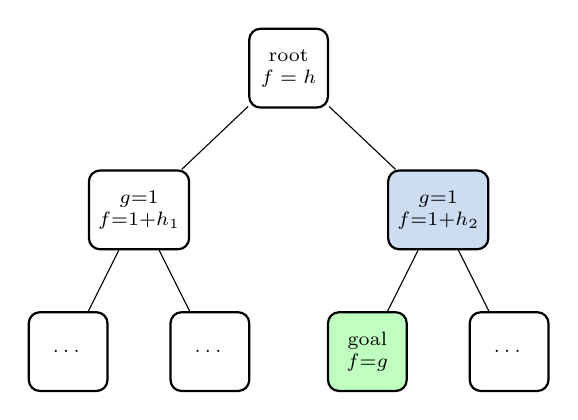
\begin{tikzpicture}[level distance=18mm,
  level 1/.style={sibling distance=38mm},
  level 2/.style={sibling distance=18mm},
  every node/.style={draw,thick,rounded corners,align=center,
                     minimum size=10mm,font=\scriptsize}]
  \node {root\\ $f=h$}
    child {node {$g{=}1$\\ $f{=}1{+}h_1$}
      child {node {$\dots$}}
      child {node {$\dots$}}
    }
    child {node[fill=dauphineblue!20] {$g{=}1$\\ $f{=}1{+}h_2$}
      child {node[fill=green!25] {goal\\ $f{=}g$}}
      child {node {$\dots$}}
    };
\end{tikzpicture}
\caption{A small A* search tree. The frontier is ordered by $f = g + h$. The
shaded node has the smallest $f$, so it is expanded first and reaches the goal.}
\label{fig:tree}
\end{figure}

\subsection{The solve method}

The \texttt{solve} method follows the A* pseudo code of Lecture 2. It uses the
frontier and the explored set. It tests the goal when a node is popped, which
keeps the search optimal. It rebuilds the plan by walking the parent chain and
reading the action of each node. Algorithm~\ref{alg:astar} shows the method.

\begin{algorithm}[H]
\caption{The A* search loop, as implemented in solve.}
\label{alg:astar}
\begin{lstlisting}[style=pseudo]
push the root state into the frontier
while the frontier is not empty:
    node = frontier.pop()                 # smallest f = g + h
    if node already expanded with a smaller g: continue
    add node to the explored set
    if node is the goal: return the plan (walk the parent chain)
    for each child in node.expand():      # the 12 turns
        if child already expanded with a smaller g: continue
        frontier.push(child)
return failure
\end{lstlisting}
\end{algorithm}

\subsection{Reconstructing the solution}

When the goal is found, we follow the parent links from the goal to the root. At
each step we read the action that produced the node. We reverse the order. This
gives the list of moves from the start to the solved cube. The \texttt{solve}
method returns this list as strings, such as "R" or "U'".

\subsection{Why A* is optimal}

The course states that A* is optimal when the heuristic is admissible. The idea
is simple. A* tests the goal only when a node leaves the frontier with the
smallest $f$. Suppose this goal node has cost $g$. Because the goal is reached,
$h$ is zero there, so $f = g$. Any other node $n$ still in the frontier has
$f(n) = g(n) + h(n)$. Since $h$ never overestimates, $f(n)$ is a lower bound on
the cost of any solution through $n$. As $n$ was not chosen, $f(n) \ge g$. So no
cheaper solution can exist. The first goal popped is therefore optimal. We also
keep an explored set, so a configuration reached again by a longer path is
skipped, which is the graph version of A* from the course.

\subsection{Data structures}

The frontier is a priority queue ordered by $f$. Java does not offer a cheap way
to lower the key of an element already in the queue. So when a better path to a
configuration appears, we push the new entry and mark the old one as out of date.
Out of date entries are skipped when they are popped. The explored set is a hash
map from a configuration to its best known cost. Both structures compare states
by their cube, so they detect repeated configurations and keep the search from
looping.

% ======================================================================
\section{Heuristics}

A heuristic must be admissible to keep A* optimal. Both of our heuristics come
from a relaxation of the problem, as in the tutorial on informed search. A
relaxation removes some rules, so its optimal cost is a lower bound on the real
cost.

\subsection{HeuristicCube: the piece relaxation}

This heuristic assumes that each piece moves on its own. A piece is a corner with
three stickers or an edge with two stickers. The six centers never move. A piece
is well placed when all of its stickers are on their target faces. A single turn
moves four corners and four edges at once. So one turn can fix at most four
corners and at most four edges. The number of remaining moves is therefore at
least
\[
h_{\text{cube}} = \max\left(
\left\lceil \frac{\text{misplaced corners}}{4} \right\rceil,\;
\left\lceil \frac{\text{misplaced edges}}{4} \right\rceil
\right).
\]
The maximum of two lower bounds is still a lower bound, so this heuristic is
admissible.

\subsection{HeuristicLabel: the sticker relaxation}

This heuristic assumes that each sticker moves on its own. A sticker only needs to
reach its correct face. We measure the 3D Manhattan distance from its face to its
target face, counted in quarter turns. The distance is 0 on the correct face, 1
on an adjacent face, and 2 on the opposite face. We sum this distance over all 54
stickers. We then divide by the number of stickers that can change face in one
turn, which is twelve.
\[
h_{\text{label}} = \frac{1}{12} \sum_{s=1}^{54} d(s).
\]
One turn moves twelve belt stickers. Each one moves to an adjacent face, so it
cuts its distance by at most one. The total distance drops by at most twelve per
move. The number of remaining moves is therefore at least the sum divided by
twelve. So this heuristic is admissible.

\subsection{Checking admissibility}

We checked both heuristics by tests. On a cube scrambled with $k$ random moves,
the heuristic must not exceed $k$, because undoing the scramble takes at most $k$
moves. We ran this check for many seeds and depths. The heuristic value was always
at most $k$. We also checked that both heuristics return zero on the solved cube.
A stronger check appears in the experiments: A* with these heuristics returns the
same solution length as the uniform cost search, which proves that they keep the
search optimal.

\subsection{A small worked example}

Take a solved cube and apply one move, the turn F. This move sends twelve belt
stickers to an adjacent face. For the sticker heuristic each of these twelve
stickers now sits on a face next to its target, so its distance is one. The sum
is twelve, and $h_{\text{label}} = 12 / 12 = 1$. The true cost is also one, so the
estimate is exact here. For the piece heuristic this same move misplaces four
corners and four edges. So the value is $\max(\lceil 4/4 \rceil, \lceil 4/4
\rceil) = 1$. Both heuristics agree with the real cost of one move.

\subsection{Comparing the two heuristics}

A heuristic $h_a$ dominates another $h_b$ when $h_a(n) \ge h_b(n)$ for every
state $n$, while both stay admissible. A dominating heuristic is never worse, and
it usually expands fewer states. In our tests the sticker heuristic gives larger
values on most scrambled cubes, so it guides the search better. The experiments
in Section 6 confirm this: the sticker heuristic expands fewer states than the
piece heuristic at the same depth. Both remain admissible, so both keep A*
optimal.

% ======================================================================
\section{Experiments}

\subsection{Setup}

We measured three strategies. The first is the uniform cost search, where $h = 0$.
The second is A* with the piece heuristic. The third is A* with the sticker
heuristic. For each strategy and each scramble depth, we solved several cubes. We
recorded the success rate, the average number of expanded states, the average
time, and the average solution length. A run fails when it expands more states
than a fixed limit. The seeds are fixed, so the numbers can be reproduced.

\subsection{Results}

Table~\ref{tab:results} reports the main numbers. The pattern is clear. The
uniform cost search blows up around depth seven. It expands hundreds of thousands
of states at depth six. It then fails at depth seven and eight under the limit.
Both heuristics scale much further. The sticker heuristic is the strongest here.
It expands far fewer states than the piece heuristic.

\begin{table}[H]
\centering
\small
\begin{tabular}{r|rr|rr|rr}
\toprule
 & \multicolumn{2}{c|}{UCS ($h=0$)} & \multicolumn{2}{c|}{A* HeuristicCube} & \multicolumn{2}{c}{A* HeuristicLabel} \\
Depth & expanded & time (ms) & expanded & time (ms) & expanded & time (ms) \\
\midrule
4 & 6\,818 & 26 & 8 & 0.1 & 14 & 0.2 \\
5 & 20\,599 & 86 & 64 & 0.7 & 40 & 0.9 \\
6 & 503\,575 & 3\,170 & 450 & 5.2 & 400 & 5.7 \\
7 & fails & n/a & 6\,953 & 66 & 1\,597 & 16 \\
8 & fails & n/a & 26\,304 & 207 & 5\,793 & 56 \\
\bottomrule
\end{tabular}
\caption{Average expanded states and time per strategy and scramble depth. UCS
fails from depth seven under the node limit.}
\label{tab:results}
\end{table}

Figure~\ref{fig:plot} draws the number of expanded states on a logarithmic
scale. The gap between the uniform cost search and A* grows very fast. At depth
six the difference is about three orders of magnitude. The two A* curves stay low
and close, with the sticker heuristic slightly below the piece heuristic.

\begin{figure}[H]
\centering
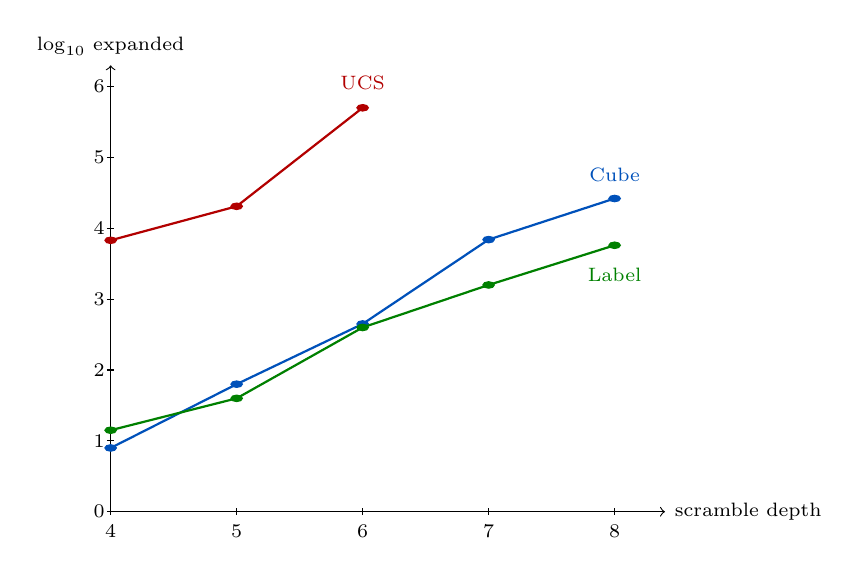
\begin{tikzpicture}[scale=1.0]
  % axes
  \def\xmin{4} \def\xmax{8}
  % log10 values of expanded counts, mapped to y
  % UCS: 4->3.83, 5->4.31, 6->5.70 ; Cube: 4->0.9,5->1.8,6->2.65,7->3.84,8->4.42 ; Label: 4->1.15,5->1.6,6->2.6,7->3.2,8->3.76
  \begin{scope}[xscale=1.6,yscale=0.9]
    \draw[->] (4,0) -- (8.4,0) node[right]{\scriptsize scramble depth};
    \draw[->] (4,0) -- (4,6.3) node[above]{\scriptsize $\log_{10}$ expanded};
    \foreach \x in {4,5,6,7,8} \draw (\x,0.05) -- (\x,-0.05) node[below]{\scriptsize \x};
    \foreach \y in {0,1,2,3,4,5,6} \draw (3.97,\y) -- (4.03,\y) node[left]{\scriptsize \y};
    % UCS (red), only 4..6 then fails
    \draw[thick,red!70!black] (4,3.83) -- (5,4.31) -- (6,5.70);
    \node[red!70!black,font=\scriptsize] at (6.0,6.05) {UCS};
    \filldraw[red!70!black] (4,3.83) circle (1.3pt) (5,4.31) circle (1.3pt) (6,5.70) circle (1.3pt);
    % Cube (blue)
    \draw[thick,dauphineblue] (4,0.9) -- (5,1.8) -- (6,2.65) -- (7,3.84) -- (8,4.42);
    \node[dauphineblue,font=\scriptsize] at (8.0,4.75) {Cube};
    \filldraw[dauphineblue] (4,0.9) circle (1.3pt) (5,1.8) circle (1.3pt) (6,2.65) circle (1.3pt) (7,3.84) circle (1.3pt) (8,4.42) circle (1.3pt);
    % Label (green)
    \draw[thick,green!50!black] (4,1.15) -- (5,1.6) -- (6,2.6) -- (7,3.2) -- (8,3.76);
    \node[green!50!black,font=\scriptsize] at (8.0,3.35) {Label};
    \filldraw[green!50!black] (4,1.15) circle (1.3pt) (5,1.6) circle (1.3pt) (6,2.6) circle (1.3pt) (7,3.2) circle (1.3pt) (8,3.76) circle (1.3pt);
  \end{scope}
\end{tikzpicture}
\caption{Expanded states by depth, log scale. UCS grows much faster and stops at
depth six within memory. Both A* curves stay low.}
\label{fig:plot}
\end{figure}

\subsection{A complete example}

To make the result concrete, we scramble a solved cube with seven moves and solve
it with the sticker heuristic. Table~\ref{tab:example} shows the scramble, the
plan, and the search effort. The plan has seven moves, so it is optimal. We can
also see that the plan is the scramble read backward, with each move replaced by
its inverse. This is the shortest way to undo the scramble, and A* finds it.

\begin{table}[H]
\centering
\small
\begin{tabular}{ll}
\toprule
Scramble (7 moves) & \texttt{F U' L U R' D L'} \\
Solution (7 moves) & \texttt{L D' R U' L' U F'} \\
Expanded states    & 1\,110 \\
Generated states   & 12\,030 \\
Time               & about 20 ms \\
\bottomrule
\end{tabular}
\caption{A complete solve with the sticker heuristic. The plan undoes the
scramble in the optimal number of moves.}
\label{tab:example}
\end{table}

\subsection{Optimality}

The solution length is the same for the three strategies at every depth. For
example, the average length is 6.0 at depth six and 7.6 at depth eight, for all
three. This is an empirical proof that the heuristics are admissible. A heuristic
that overestimated the cost would make A* return a longer plan than the uniform
cost search. This never happens.

\subsection{Discussion}

The experiments confirm the course. First, the heuristic does not change the
answer, only the effort to find it. The plans stay optimal. Second, a good
heuristic gives huge savings. At depth six the uniform cost search expands about
$500\,000$ states, while A* expands a few hundred. Third, the sticker heuristic
dominates the piece heuristic here, because it gives finer values. Finally, A*
runs out of memory before it runs out of time, exactly as the slides state. The
limit we hit first is the number of stored states, not the clock.

\subsection{A simple optimization}

We also added one optional optimization. After a move, we never apply its inverse
right away. For example we never play U' just after U. Such a pair cancels out, so
it can never belong to an optimal solution. Skipping it keeps the search optimal
and makes the tree smaller. This option is turned off by default, so the
\texttt{solve} method stays close to the pseudo code of the course. When it is
turned on, A* expands fewer states at the same depth.

\subsection{Methodology}

We built the project with a test first method. For each class we wrote the tests
before the code. We made the tests fail, then wrote the code until they passed.
The cube tests check the algebraic invariants. The search tests check that the
plan really solves the cube and that A* matches the optimal length. In total the
project has twenty four tests, and they all pass. The code was also reviewed,
which helped us find and fix a rotation that turned the wrong way and a few
performance issues.

\subsection{Limits}

A* is still exponential in the worst case. Our solver stays fast up to about
eight or nine random moves. Beyond that, the frontier grows too large for memory.
This is a known limit of A* on the Rubik's Cube. Stronger methods exist, but they
are outside the scope of this lab.

% ======================================================================
\section{Conclusion}

We built a program that solves the Rubik's Cube with the A* algorithm. We modeled
the cube as a search problem with the five components of the course. We followed
the statement and built the classes Cube, State, Astar, StateSet,
PriorityQueueState, and the heuristics. We first ran a uniform cost search. We
then added two admissible heuristics, both from a relaxation of the problem.

The results match the theory. A* returns an optimal solution. A good heuristic
cuts the number of expanded states by several orders of magnitude. The uniform
cost search fails from about seven random moves, while A* solves more scrambled
cubes. The main limit is memory, not time. This project gave us a clear, hands on
view of informed search and of why heuristics matter.

\subsection*{Team contributions}

The three members worked together on the design and the report. The work was
shared as follows. One member focused on the cube model and the turns. One member
focused on the A* search and the data structures. One member focused on the two
heuristics and the experiments. The interface, the tests, and the writing were a
shared effort, with regular reviews between the members.

\end{document}
